%%%%%%%%%%%%%%%%%%%%%%%%%%%%%%%%%%%%%%%%%
% Beamer Presentation
% LaTeX Template
% Version 1.0 (10/11/12)
%
% This template has been downloaded from:
% http://www.LaTeXTemplates.com
%
% License:
% CC BY-NC-SA 3.0 (http://creativecommons.org/licenses/by-nc-sa/3.0/)
%
%%%%%%%%%%%%%%%%%%%%%%%%%%%%%%%%%%%%%%%%%

%----------------------------------------------------------------------------------------
%	PACKAGES AND THEMES
%----------------------------------------------------------------------------------------

\documentclass{beamer}

\mode<presentation> {

\usetheme{CambridgeUS}

\usecolortheme{dolphin}
}

\usepackage{xcolor}
\usepackage{graphicx} % Allows including images
\usepackage{booktabs} % Allows the use of \toprule, \midrule and \bottomrule in tables

%----------------------------------------------------------------------------------------
%	TITLE PAGE
%----------------------------------------------------------------------------------------

\title[Projects for Engr Math Students]{Designing Projects for Engineering Mathematics Students} % The short title appears at the bottom of every slide, the full title is only on the title page

\author{Jeremy L Thompson} % Your name
\institute[USAFA] % Your institution as it will appear on the bottom of every slide, may be shorthand to save space
{United States Air Force Academy \\ % Your institution for the title page
\medskip
\textit{jeremy.thompson@usafa.edu} % Your email address
}
\date{\today} % Date, can be changed to a custom date

\begin{document}

\begin{frame}
\titlepage % Print the title page as the first slide
\end{frame}

%------------------------------------------------

\begin{frame}
\begin{center}
\frametitle{Overview}

Projects are often an important component in mathematics courses for engineering students. In this talk, I discuss a series of projects I designed for two courses, Calculus III and Engineering Mathematics (Systems of DEs and Introduction to PDEs). I focus on project goals and where these projects appeared to do well or fall short.

\end{center}
\end{frame}
 
%------------------------------------------------

\begin{frame}
\frametitle{Overview} % Table of contents slide, comment this block out to remove it
\tableofcontents % Throughout your presentation, if you choose to use \section{} and \subsection{} commands, these will automatically be printed on this slide as an overview of your presentation
\end{frame}

%----------------------------------------------------------------------------------------
%	PRESENTATION SLIDES
%----------------------------------------------------------------------------------------

%------------------------------------------------
\section{Background}
%------------------------------------------------

\begin{frame}
\begin{center}
\frametitle{Engineering Math at USAFA}

Engineering Math Sequence

\begin{enumerate}

\item Calculus I (differential calculus)

\item Calculus II (integral calculus)

\item Calculus III (multivariate and vector calculus)

\item Differential Equations

\item Engineering Mathematics (systems of DEs, PDEs, numerical methods, vector calculus)

\end{enumerate}

\end{center}
\end{frame}

%------------------------------------------------

\begin{frame}
\begin{center}
\frametitle{Engineering Math at USAFA}

Engineering Math Sequence

\begin{enumerate}

\item Calculus I (differential calculus)

\item Calculus II (integral calculus)

\item {\color{red}Calculus III} (multivariate and vector calculus)

\item Differential Equations

\item {\color{red}Engineering Mathematics} (systems of DEs, PDEs, numerical methods, vector calculus)

\end{enumerate}

\end{center}
\end{frame}
 
%------------------------------------------------
\section{Projects}
%------------------------------------------------

\begin{frame}
\begin{center}
\frametitle{2 Courses, 3 Projects}

3 projects designed to incrementally build student capability\\

~\\

1 project in Calculus III\\

~\\

2 projects in Engineering Mathematics

\end{center}
\end{frame}

%------------------------------------------------

\begin{frame}
\begin{center}
\frametitle{Calculus III}

Lagrange Multipliers, optimize construction\\

~\\

Students walked through process

\begin{enumerate}

\item Optimize simpler version

\item Optimize complex version

\end{enumerate}

Deliverables

\begin{enumerate}

\item Points paper justifying modeling

\item Points paper summarizing results and commented Mathematica code

\end{enumerate}

\end{center}
\end{frame}

%------------------------------------------------

\begin{frame}
\begin{center}
\frametitle{Calculus III}

\begin{figure}

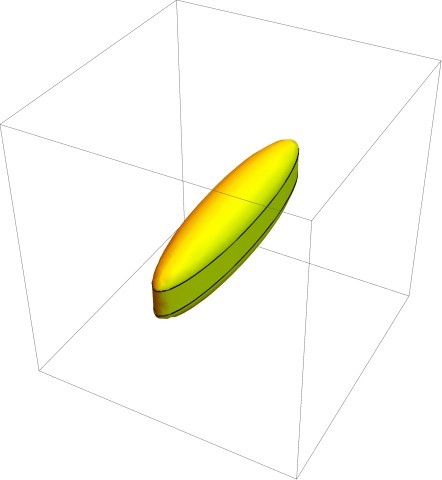
\includegraphics[width = 0.4 \linewidth]{CalcIIISol1.jpg}
\hspace{7.5 mm}
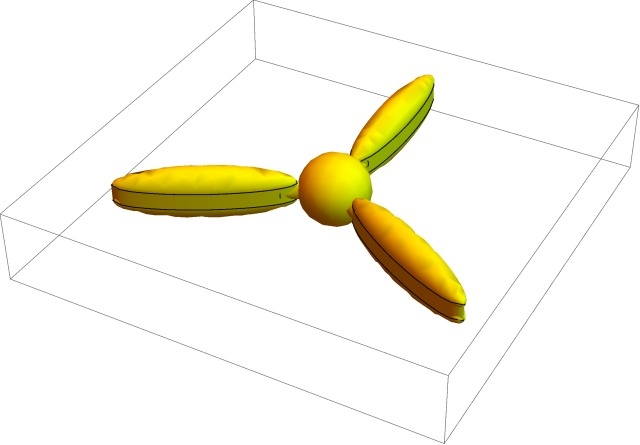
\includegraphics[width = 0.4 \linewidth]{CalcIIISol2.jpg}

\end{figure}

\end{center}
\end{frame}

%------------------------------------------------

\begin{frame}
\begin{center}
\frametitle{Systems of ODEs}

Compare analytic/numerical solutions to nonhomogeneous linear systems\\

~\\

Jacobian analysis/numerical solution to nonlinear system\\

~\\

Less step by step instructions, close to class exercises\\

~\\

Deliverables

\begin{enumerate}

\item Draft technical report for peer review

\item Peer review

\item Final technical report with commented Mathematica and Matlab code

\end{enumerate}

\end{center}
\end{frame}

%------------------------------------------------

\begin{frame}
\begin{center}
\frametitle{Systems of ODEs}

\begin{figure}

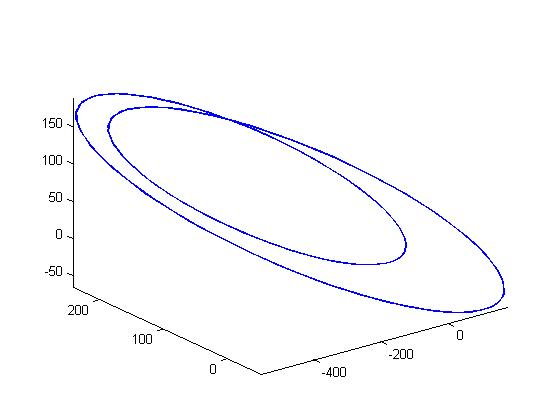
\includegraphics[width = 0.4 \linewidth]{ODESol1.jpg}
\hspace{7.5 mm}
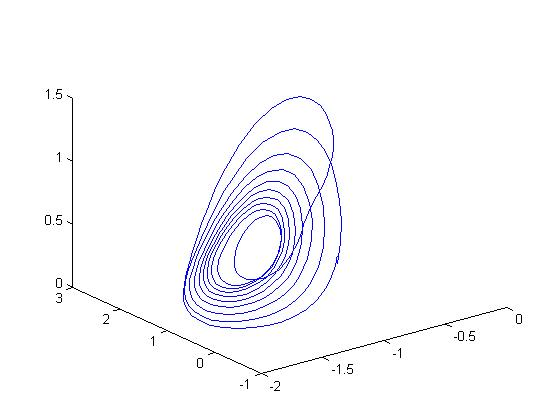
\includegraphics[width = 0.4 \linewidth]{ODESol2.jpg}

\end{figure}

\end{center}
\end{frame}

%------------------------------------------------

\begin{frame}
\begin{center}
\frametitle{PDEs}

Analytic/numerical solution to 2D heat equation\\

~\\

Mapping solution to a torus\\

~\\

Extension from class exercises (1D heat and 2D Laplace)\\

~\\

Deliverables

\begin{enumerate}

\item Draft technical report for peer review

\item Peer review

\item Final technical report with commented Mathematica and Matlab code

\end{enumerate}

\end{center}
\end{frame}

%------------------------------------------------

\begin{frame}
\begin{center}
\frametitle{Systems of ODEs}

\begin{figure}

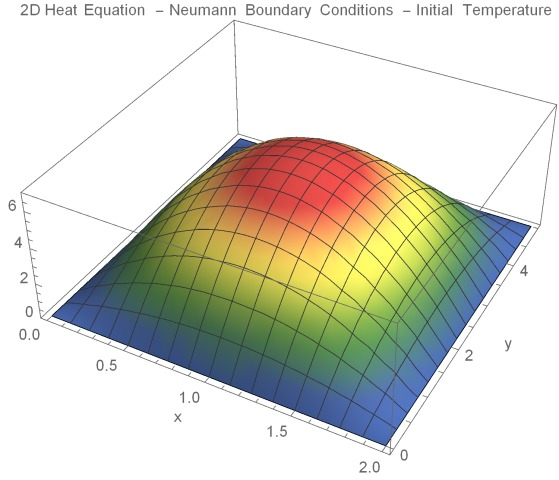
\includegraphics[width = 0.4 \linewidth]{PDESol1.jpg}
\hspace{7.5 mm}
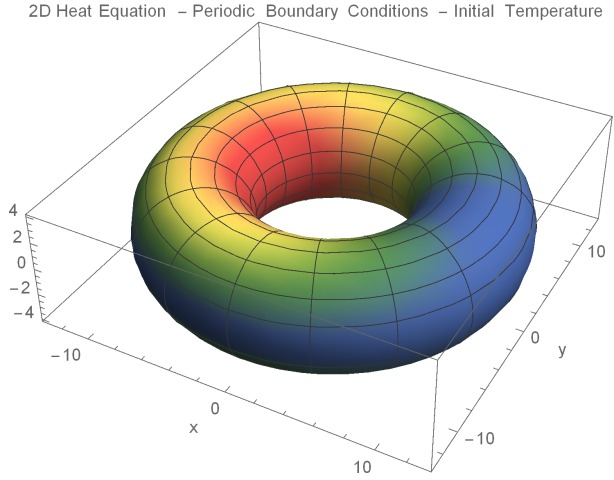
\includegraphics[width = 0.4 \linewidth]{PDESol2.jpg}

\end{figure}

\end{center}
\end{frame}

%------------------------------------------------
\section{Lessons Learned}
%------------------------------------------------

\begin{frame}
\begin{center}
\frametitle{Lessons Learned}

Calculus III Project

\begin{enumerate}

\item Starting with simpler model helps

\item Check values let students validate modeling

\end{enumerate}

System of ODEs Project

\begin{enumerate}

\item Juniors/Sophomores still need very clear instructions

\item Peer review needs guidelines

\item Too much repetition in tasks detrimental

\end{enumerate}

PDEs Project

\begin{enumerate}

\item Commenting code a common issue

\item Varying levels of success following extensions on in class exercises

\end{enumerate}

\end{center}
\end{frame}

%------------------------------------------------
\section{}
%------------------------------------------------

\begin{frame}[noframenumbering]
\titlepage % Print the title page
\end{frame}

%------------------------------------------------

%----------------------------------------------------------------------------------------

\end{document} 